
\begin{frame}[fragile]
\frametitle{NumPy module}

\begin{itemize}
\item Specific module for numerical simulations.
\item Very excellent for array manipulation.
\item Documentation from \url{https://www.numpy.org/}
\end{itemize}

%\newcommand{\newfilename}{py-matplotlib.py}
%\lstinputlisting[language=Python, firstline=1, lastline=7]{../py-matplotlib.py}
%file: \newfilename

\end{frame}

%-------------------------------------------------------------------------------

\begin{frame}[fragile]
\frametitle{SciPy module}

\begin{itemize}
\item Scientific calculations module.
\item Lots of functions for scientific computation.
\item Documentation from \url{https://www.scipy.org/}
\item Specific manuals \url{https://docs.scipy.org/doc/scipy-1.3.0/reference/}
\end{itemize}

%\newcommand{\newfilename}{py-matplotlib.py}
%\lstinputlisting[language=Python, firstline=1, lastline=7]{../py-matplotlib.py}
%file: \newfilename

\end{frame}

%--------------------------------------------------------------------------------

\begin{frame}[fragile]
\frametitle{Matplotlib module}

\begin{itemize}
\item Very efficient module for plotting almost everything.
\item Capable for plotting graphs and images.
\item Documentation from \url{https://matplotlib.org/3.1.0/index.html}
\end{itemize}

\newcommand{\newfilename}{py-matplotlib.py}
\lstinputlisting[language=Python, firstline=1, lastline=7]{../py-matplotlib.py}
file: \newfilename

\end{frame}

%-------------------------------------------------------------------------------

\begin{frame}[fragile]
\frametitle{pandas module}

\begin{itemize}
\item Python data analysis module.
\item The go-to module for data analysis.
\item Documentation from \url{https://pandas.pydata.org/}
\end{itemize}

\end{frame}

%-------------------------------------------------------------------------------

\begin{frame}[fragile]
\frametitle{Numba module}

\begin{itemize}
\item Python module for high performance computing.
\item Just-In-Time (JIT) compiler for faster computation.
\item Documentation from \url{https://numba.pydata.org/}
\end{itemize}

%\newcommand{\newfilename}{py-matplotlib.py}
%\lstinputlisting[language=Python, firstline=1, lastline=7]{../py-matplotlib.py}
%file: \newfilename

\end{frame}

%-------------------------------------------------------------------------------

\begin{frame}[fragile]
\frametitle{*Numba with CUDA}

\begin{itemize}
\item GPU computing implementation using Numba-CUDA.
\item Very common in AI and DeepLearning implementation.
\item Example code:
\end{itemize}

\newcommand{\newfilename}{py-numba-cuda.py}
\lstinputlisting[language=Python, firstline=1, lastline=4]{../py-numba-cuda.py}
file: \newfilename

*Special settings are required.
\end{frame}
%---------------------------------------------------------------------------------

\begin{frame}[fragile]
\frametitle{Numba with CUDA}
\newcommand{\newfilename}{py-numba-cuda.py}

\begin{itemize}
\item Example output for device detection.
\end{itemize}
\begin{figure}
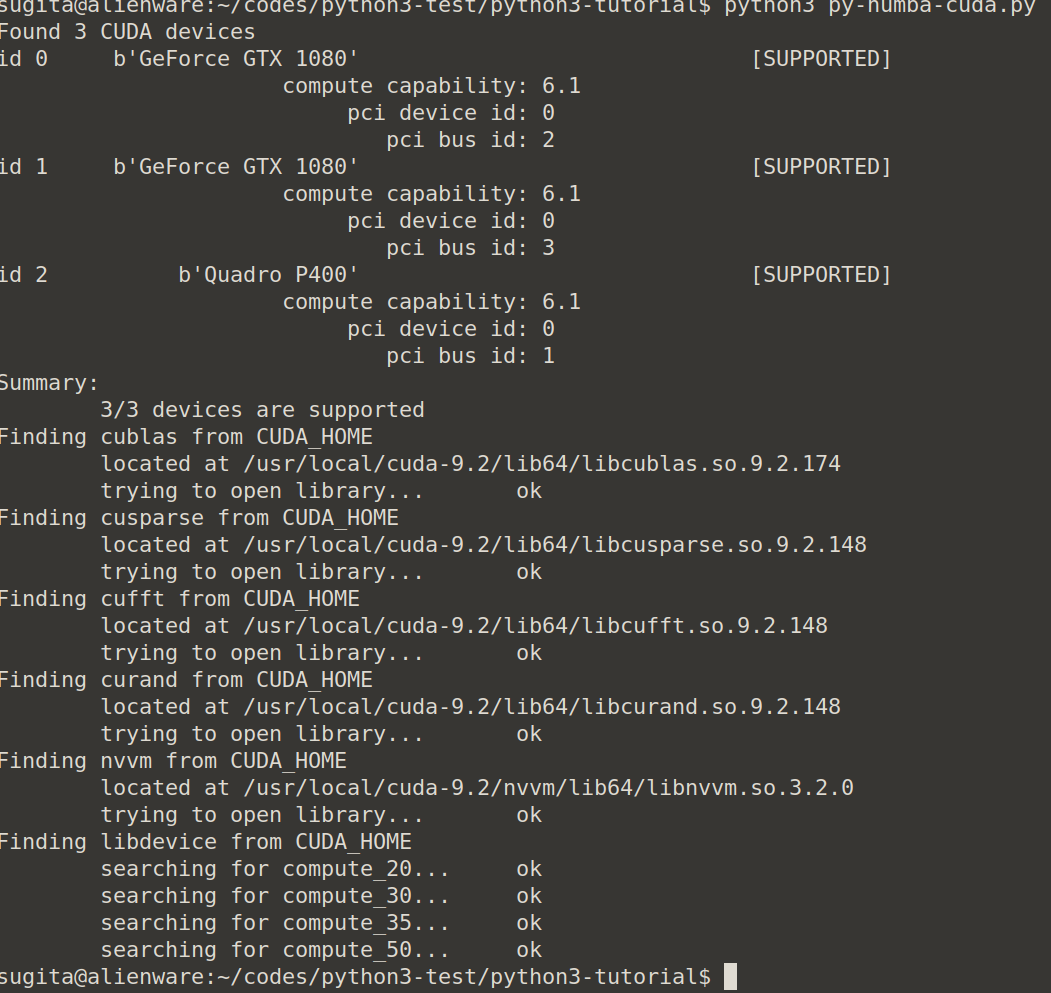
\includegraphics[width=0.5\textwidth]{dev-numba.png}
\caption{Numba's device detection.}
\end{figure}
file: \newfilename
\end{frame}

%-------------------------------------------------------------------------------

\begin{frame}[fragile]
\frametitle{Numba with CUDA}
\begin{itemize}
\item Example for CUDA kernel using numba
\end{itemize}
\newcommand{\newfilename}{py-numba-cuda-mxm.py}
\lstinputlisting[language=Python, firstline=6, lastline=16]{../py-numba-cuda-mxm.py}
file: \newfilename
\end{frame}

%-------------------------------------------------------------------------------